\section{ P-A*mbush: Ambush with Priorities assignment method P}

Without a strategy that decides which agent calculates it's path 
first, routes that are inconvenient could be chosen, because the 
algorithm doesn't take in account the agent's state in the game. 
For example, if agent $i$ is the closest one to the goal, it could 
be beneficial to make $i$ perform the path computing first. 
This way the agent won't end up tacking a long route to generate 
ambush, wasting an opportunity to catch the wanted element,
 while an agent that was further away takes the most direct way.
 
 For this work two a simple P method is proposed based on 
 the real distance between the agents an the goal. This is
 because the positions of the agents are a very general and
 intuitive property that defines the advantage that an element
 could have over another.
 Other character properties like strength, remaining
 life, stamina, and any others could be used in this method to 
 generate the desired group strategy while performing \ambush.
 
 Figure \ref{fig:grids} shows the path that three agents would take when 
 performing \ambush\ (left Image) and \pambush\ with
 real distance (right Image).
 The circles represent the agents, the numbers inside them represent the order
 in which each agent computes the path it will take and the black cross represents
 the goal.
 
 \begin{figure}[htp]
\centerline{
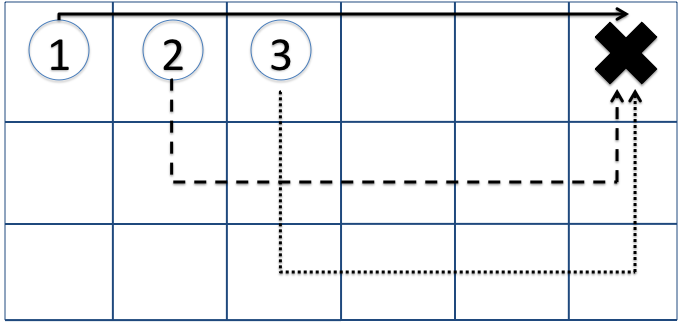
\includegraphics[width=0.4\columnwidth]{figures/ambush_grid.png}
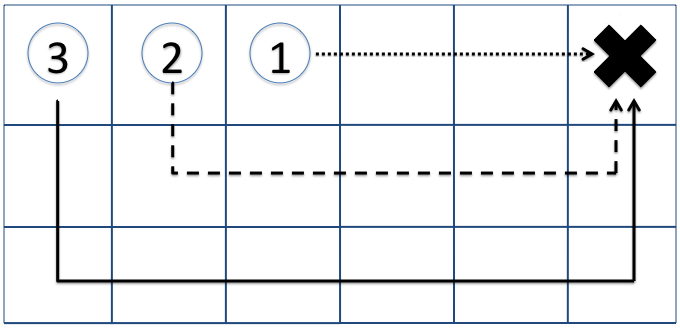
\includegraphics[width=0.4\columnwidth]{figures/priorities_grid.png}
}
\caption{The numbers represent the order in which the agents
are calculating the path.
Up: Performance of \ambush. Since it does not take the distance to the
              goal into account, the agent that is closer to the goal, takes a longer path.
              Down: Performance of \pambush\ using $A^*$'s distance. The agent that
              can reach the goal first using the path given by \astar has the top priority for
              calculating the path, the second closest by this distance goes afterwards, and so on.}
\label{fig:grids}
\end{figure}

When using \pambush, the behaviours of the agents look more intelligent, 
since the one that is closer to the goal is taking the most direct path to reach it, instead
of the circling around like the one performing \ambush\ does.

Other advantage that \pambush\ displays is that  the
goal will always be reached in the minimum time possible by 
one of the agents. Thus,  this algorithm shows qualitative
improvements over  \ambush.

Although the cost of computing \pambush\ with real distance is
bigger than computing \ambush\ for one agent, the amortized
cost invested to calculate \pambush\ for each agent equals
\ambush's amortized cost.
However, having agents perform \textit{P-A}$^*$\textit{mbush} with real distance 
would decrease the frame rate because of the involved constants.
Therefore, using the euclidean 
distance is proposed as a good middle. It will not perform as well as 
the one using $A^*$'s distance, but also, it's computational cost will
not differ from the one in \ambush.